%	CHAP Simulate Datasets%----------------------------------------------------------------------------------------

\chapterimage{blue-chapter-head_4-reduced.pdf} % Chapter heading image

\chapter{Simulating Datasets}\label{chap:SimulatingDatasets}

\section{Why simulating datasets}

Simulated datasets are useful to check that analyses work as expected. MetaR provides a \texttt{Simulate Dataset} command that allows to simulate datasets starting from a few assumptions and parameter values. This approach could be also beneficial at experimental design time to validate certain assumptions before running (expensive) experiments.

  In order to use the command inside an Analysis script, the \textit{simulation} language (\texttt{org\allowbreak.campagnelab\allowbreak.metaR\allowbreak.simulation}) has to be imported in the current model (use \keys{\cmd+L} and select the language from the list). Figure~\ref{fig:NewSimulateStatement} shows a new \texttt{simulate dataset} statement.

\begin{figure}[h!tbp]
  \centering
  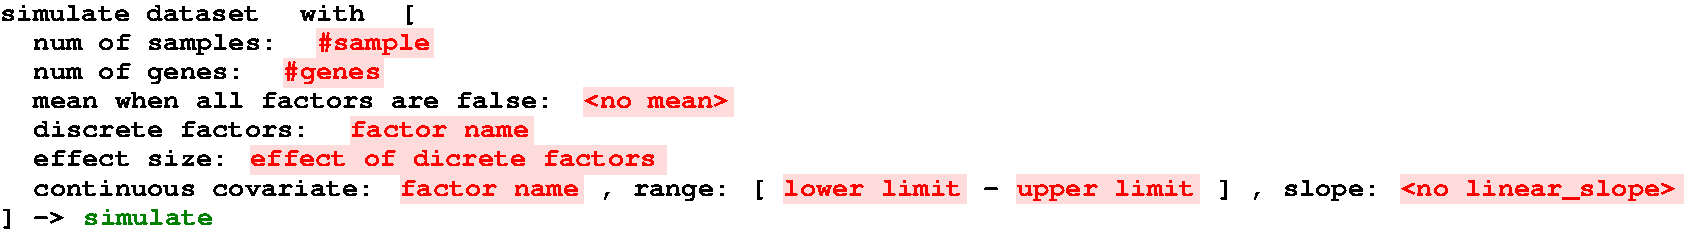
\includegraphics[width=\figWidthWide]{figures/NewSimulateStatement.pdf}
\caption[New Simulate Dataset Statement.]{\textbf{New Simulate Dataset Statement.} A new \texttt{simulate dataset} statement created after you have added the \texttt{org.campagnelab.metaR.simulation} language to the model's MPS Used Languages.}
\label{fig:NewSimulateStatement}
\end{figure}
 

\section{The Simulate Dataset Statement}
The \texttt{simulate dataset} statement is configurable and lets you create datasets that reflect different simulation scenarios.  The output dataset is represented by a \texttt{Table} node that can be then further manipulated with other MetaR statements. 

\paragraph{num of samples}
The number of samples included in the dataset. Each sample is named according to the results of the simulation. If the simulation decides that the sample name \emph{sample\_3 }has been treated with a discrete factor named \emph{LPS}, it is renamed to \emph{sample\_3\_LPS} to make it easy to identify the simulated treatment.

\paragraph{num of genes}
The number of genes included in the dataset. Each gene is renamed according to the results  of the simulation. If the simulation decides that the gene named \emph{gene\_2} is affected by a discrete factor named \emph{LPS}, it is renamed to \emph{gene\_2\_LPS} to make it easy to identify the simulated treatment.

\paragraph{mean}
The value of the mean expression level for each gene, assuming no treatment.

\paragraph{discrete factors}
List of treatments used in the simulation. About 50\% of the samples will be considered treated with each factor specified here. About 30\% of the genes will be considered affected by each factor.

\paragraph{effect of discrete factors}
The impact of each discrete factor on the data generated by the simulation

\paragraph{continuous covariate}
A covariate that will affect the value of the gene expression level. You can define the age of the covariate, its range and the slope. A value is added to the expression value of each gene equal to the product of the slope and the cofactor value. Cofactors are set for each sample using a uniform distribution. For instance, if you indicate an 'age' continous covariate between 0 and 36, each sample will be assigned an age in this range, and the value added to the expression level of the gene will be determine for each sample by multiplying the age of the sample by the slope of the 'age' cofactor.

\section{Example}

\begin{figure}[h!tbp]
  \centering
  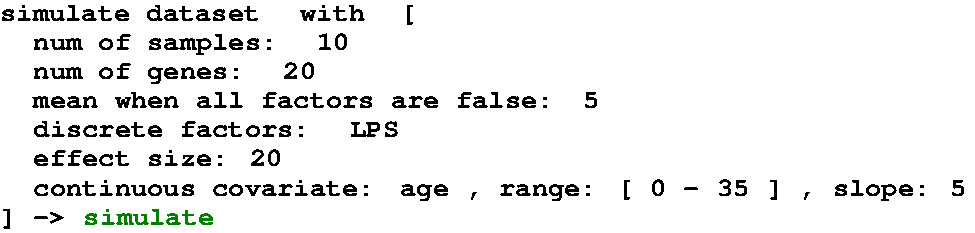
\includegraphics[width=\figWidthWide]{figures/SimulateStatementWithParameters.pdf}
\caption[SimulateDataset Example.]{\textbf{Simulate Dataset Example.} This statement will create a dataset with a single discrete factor (LPS) and a covariate factor (age) with a range of 0 to 36 (for instance, this could be the mouse age in a mouse model). }
\label{fig:SimulateDatasetExample}
\end{figure}


\begin{figure}[h!tbp]
  \centering
  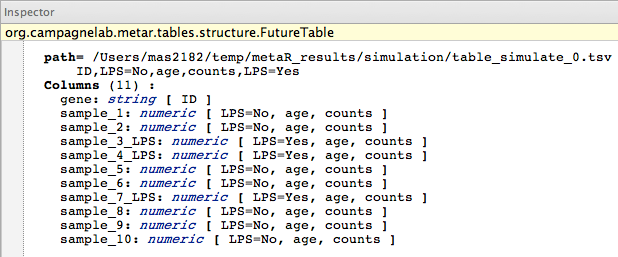
\includegraphics[width=\figWidthWide]{figures/SimulateTableInspector.png}
\caption[Preview of the Dataset Structure as Shown in the Inspector.]{\textbf{Preview of the Dataset Structure as Shown in the Inspector.}}
\label{fig:SimulateDatasetInspector}
\end{figure}

\begin{figure}[h!tbp]
  \centering
  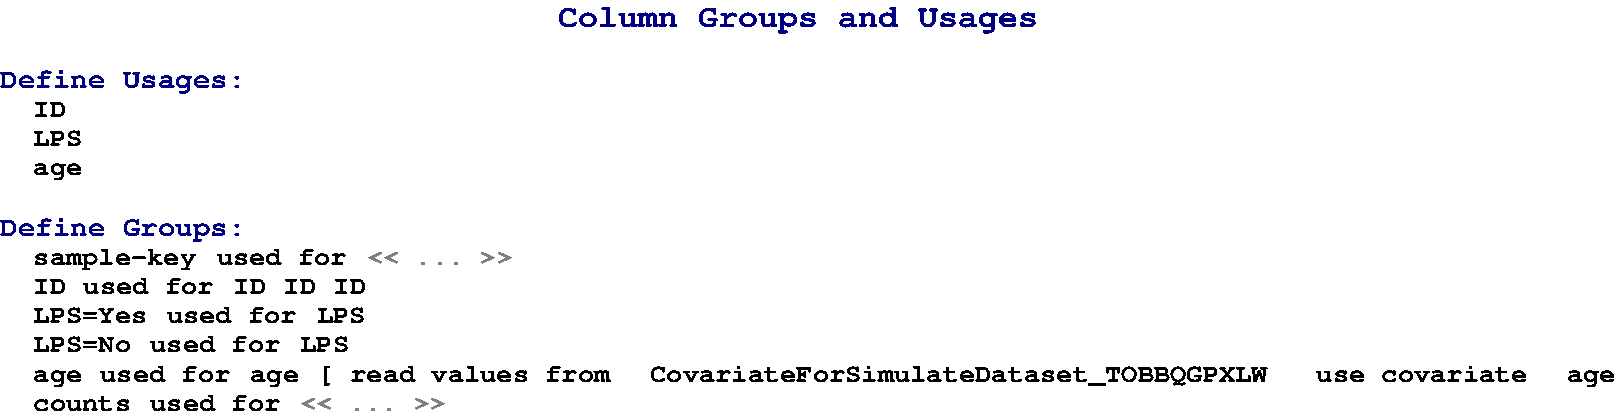
\includegraphics[width=\figWidthWide]{figures/SimulateGroups.pdf}
\caption[Column Group Annotations Created in the Model.]{\textbf{Column Group Annotations Created in the Model.}}
\label{fig:SimulateGroups}
\end{figure}

\begin{figure}[h!tbp]
  \centering
  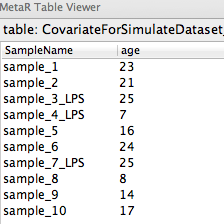
\includegraphics[width=\figWidthNarrow]{figures/SimulateCovariateTableInspector.png}
\caption[Covariate Table Generated with Simulate Dataset.]{\textbf{Covariate Table Generated with Simulate Dataset.}}
\label{fig:SimulateCovariateTableInspector}
\end{figure}


\begin{figure}[h!tbp]
  \centering
  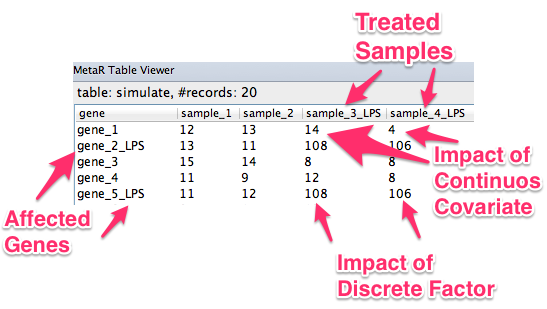
\includegraphics[width=\figWidthWide]{figures/SimulateTableViewer.png}
\caption[Table Generated with Simulate Dataset.]{\textbf{Table Generated with Simulate Dataset.} This is a partial view of the full table.}
\label{fig:SimulateDatasetViewer}
\end{figure}

